\documentclass[letterpaper,11pt]{article}
\usepackage[margin=1 in]{geometry}

\usepackage{amsmath, mathtools, comment, graphicx, fancyhdr, color, setspace, multicol, hyperref, calc}
\usepackage{tikz,tikz-3dplot,pgfplots}

%\textwidth = 6.5 in
%\textheight = 9 in
%\oddsidemargin = 0.0 in
%\evensidemargin = 0.0 in
%\topmargin = 0.0 in			 
%\headheight = 0.0 in			
%\headsep = 0.0 in
			
\parskip = 0.2in	% vertical space between paragraphs
\parindent = 0.0in  % no indent

\def\ds{\displaystyle}

\newcommand{\xfont}[1]{\[\textcolor{gray}{\mathtt{#1}}\]}

\begin{document}

\textbf{Grade this Quiz} \hfill Name: \rule{4cm}{0.01cm}

A student was asked to find the derivative of the following functions.  Mark each answer as correct or incorrect.  If the answer is wrong, explain to the student both what their error was and how to do the problem correctly.  At the top of a page, give the total score out of 10.

\begin{enumerate}
\item $f(x)=x^3+7x^2-3+\sqrt{x}$
\xfont{f'(x)=3x+14x-3+\frac{1}{2\sqrt{x}}}
\vfill
\item $g(x)=x^2\sin{x}$
\xfont{g'(x)=2x\cos{x}}
\vfill
\item $h(x)=\tan^2 x$
\xfont{h'(x)=2\tan{x} \cdot \sec^2 x}
\vfill
\item $m(x)=\tan{(x^2)}$
\xfont{m'(x)=2\tan{x}\sec^2 x}
\vfill
\item $n(x)=e^{\sec{x}}$
\xfont{n'(x)=e^{\sec{x}\tan{x}}}
\vfill
\newpage
\item $p(x)=2^x$
\xfont{p'(x)=x \cdot 2^{x-1}}
\vfill
\item $q(x)=\dfrac{x}{\ln{x}}$
\xfont{q'(x)=\frac{\ln{x}-1}{(\ln{x})^2}}
\vfill
\item $\ds l(x)=\sqrt{\cos{\left(x^3\right)}}$
\xfont{l'(x)=\frac{1}{2\sqrt{\cos{\left(x^3\right)}}} \cdot 3x^2}
\vfill
\item $h(x)f(g(x))$
\xfont{\left(h(x)f(g(x))\right)'=h'(x)f(g(x))+h(x) \cdot f'(g(x))(g'(x))}
\vfill
\begin{minipage}{0.65\textwidth}
\item Find $h'(2)$. Assume $f(1)=2, f(2)=0, f'(1)=3, f'(2)=4$.
\\
$g(x)$ is given by the graph to the right.
\end{minipage}
\begin{minipage}{0.25\textwidth}
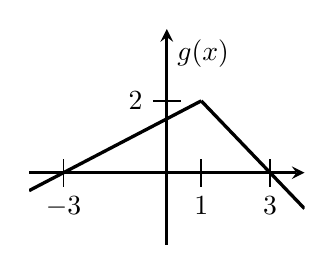
\begin{tikzpicture}
\begin{axis}[
    ylabel=$g(x)$,
   	xmin=-4, xmax=4,
	ymin=-2, ymax=4,
	major tick length={10},  tick style={semithick,color=black},
	xtick={-3,1, 3}, ytick={2},
	line width=1pt,
 	axis lines=center, height=1.7 in, width=2 in, grid=none
	]
    \addplot [black, smooth, very thick, samples=2, domain=1:4] {-x+3};
    \addplot [black, smooth, very thick, samples=2, domain=-4:1] {.5*x+3/2};
\end{axis}
\end{tikzpicture}
\end{minipage}
\vspace{-.2in}
\begin{enumerate}
\item $h(x)=f(x)g(x)$
\xfont{h'(2)=f(2) \cdot g'(2)+f'(2) \cdot g(2) = 0\cdot-1+4\cdot1=4}
\vfill
\item $h(x)=g(f(x))$
\xfont{h'(2)=g'(2) \cdot f'(2)=-1\cdot4=-4}
\vfill
\end{enumerate}
\end{enumerate}

\end{document}
